\chapter{Reti Neurali}

In questo capitolo verrà illustrato lo strumento principale utilizzato per lo sviluppo di un metodo di text localization, partendo dapprima dagli albori delle reti neurali, passando per i vari sviluppi negli anni nei vari campi, fino ad arrivare alla struttura alla base del nostro metodo.

\section{Reti Neurali Artificiali}

Le \textit{reti neurali artificali} possono essere definite come un modello matematico ispirato alle reti neurali biologiche, costituito da neuroni artificali interconnessi e da processi che dettano il cambiamento della propria struttura in base a informazioni che scorrono attraverso la rete durante la cosiddetta fase di apprendimento.

Il primo accenno al termine si deve a McCulloch e Pitts~\cite{McCulloch1943} che nel 1943 introdussero un combinatore lineare a soglia, esemplificato nella figura~\ref{fig:TLU}, in grado di ricreare funzioni booleane.

\begin{figure}[H]
	\centering
	\begin{equation*}
		\begin{aligned}[c]
			TLU(\vec{x}) &= \phi \bigg( \sum_{i=1}^{n}{w_{i} \cdot x_{i}} \bigg) \\
			\phi(x) &= x - \theta \geq 0
		\end{aligned}
		\quad
		\begin{aligned}[c]
			n &= 2 \\
			\theta &= 1.5 \\
		\end{aligned}
		\quad
		\begin{aligned}[c]
			w_{1} &= 1.0 \\
			w_{2} &= 1.0
		\end{aligned}
	\end{equation*}
	\caption{Threshold Logic Unit con relativi parametri per l'implementazione dell'and logico.}
\label{fig:TLU}
\end{figure}

Questo però non era che un semplice modello statico incapace di apprendere.
L'intuizione che diede vita ad una gran varietà d studi riguardando metodi di apprendimento automatico si deve infatti a D.O. Hebb~\cite{Hebb} il quale nel 1949 ipotizzò come l'apprendimento negli esseri viventi non fosse altro che un meccanismo di plasticità sinaptica, ovvero una modifica di intensità delle relazioni fra neuroni in base agli impulsi che li attraversano.

\subsection{Perceptron}
F. Rosenblatt ideò nel 1958 il \textit{Perceptron}\cite{rosenblatt1958perceptron}, un classificatore binario lineare, oggi considerato la più semplice rete neurale \textit{feed-forward}.

Il Perceptron può essere modellato come segue:
\begin{equation*}
	\begin{aligned}[c]
		y = f(x) =
			\begin{cases}
				1 &\text{se } w\vec{x} > 0 \\
				0 &\text{altrimenti}
			\end{cases}
	\end{aligned}
\end{equation*}

dove si incorpora un valore scalare di \textit{bias} con 
\begin{equation*}
	\begin{aligned}[c]
		w = \begin{bmatrix}
			w_{1} & \cdots & w_{d} & b
		\end{bmatrix}
	\end{aligned}
	\quad
	\begin{aligned}[c]
		\vec{x} = \begin{bmatrix}
			x_{1} \\
			\vdots \\
			x_{d} \\
			1
		\end{bmatrix}
	\end{aligned}
\end{equation*}

Si parte dunque da un dataset $D = \{(x^{(1)},g^{(1)}),\ldots, (x^{(n)},g^{(n)})\}$ formato da $n$ campioni $x^{(i)} \in \mathbb{R}^{d}$, vettori delle feature $d$-dimensionali, e $g^{(i)}$ valore di output desiderato per $f(x^{(i)})$. L'algoritmo è descritto di seguito:

\begin{enumerate}
	\item
		Inizializzazione del vettore $w$ con valori nulli o randomici tendenti a zero.
	\item
		Per ogni campione $i$ nel dataset $D$:
		\begin{enumerate}
			\item
				Calcolare $y$ al tempo corrente $t$: \\
				$y^{(i)}(t) = f[w(t) \cdot \vec{x}^{(i)}]$
			\item
				Aggiornare i valori di $w$ al nuovo tempo $t+1$: \\
				$\forall j \quad w_{j}(t+1) = w_{j}(t) + (g^{(i)} - y^{(i)}(t))x^{(i)}_{j}$
	\item
		Ripetere dal punto 2 per minimizzare $\frac{1}{n}\sum\limits_{i=1}^{n}|g^{(i)} - y^{(i)}(t)|$
		\end{enumerate}
\end{enumerate}

\subsection{Backpropagatin}
Dal 1969 la ricerca si bloccò con la dimostrazione da parte di Minsky e Papert~\cite{minsky1972} dell'impossibilità di risolvere problemi con soluzioni non separabili linearmente.
Negli anni a seguire le reti neurali vennero presto dimenticate a favore di altri modelli, come le Support Vector Machine, al tempo più efficaci nell'ambito del machine learning.\par
Nonostante questo nel 1975 venne introdotto da parte di Paul Werbos l'algoritmo per la cosiddetta \textit{backpropagation} il quale rimane tutt'oggi un ingranaggio principale per il funzionamento della gran parte delle reti neurali.

Sia $N$ una rete neurale con $e$ connessioni, $m$ input, $n$ output, $p$ osservazioni ed $E$ una funzione di costo da ottimizzare. Avremo dunque:
\begin{equation*}
	\begin{aligned}[c]
		x^{(1)},\dots,x^{(p)} \\
		y^{(1)},\dots,y^{(p)} \\
		w^{(0)},\dots,w^{(p)} \\
	\end{aligned}
	\quad
	\left.\begin{aligned}[c]
		\text{vettori di input in } &\mathbb{R}^m \\
		\text{vettori di output in } &\mathbb{R}^n \\
		\text{vettori dei pesi in } &\mathbb{R}^e
	\end{aligned}\quad \right\}
	\;
	\begin{aligned}[c]
		&y &=& &f_{N}(x,w) \\
		&E &\colon& &\mathbb{R}^{n \times n} \rightarrow \mathbb{R}
	\end{aligned}
\end{equation*}

L'output dell'algoritmo è dato da un nuovo vettore dei pesi ottenuto con il metodo del gradiente, calcolato di conseguenza dalla derivata della funzione di costo rispetto a $w$:
$$
\frac{d E}{d w}
$$

Per una serie di input perciò, partendo dal vettore $w^{(0)}$ inizializzato con valori prossimi a zero, si calcola $E(y^{(i)}, f(x^{(i)}, w^{(i-1)}))$ iterativamente ponendo $w^{(i)}$ uguale all'output dell'algoritmo alla fine di ogni iterazione.

\subsection{Multilayer Perceptron}
\label{subsec:mlp}

Partendo dai concetti precedentemente presentati passeremo ora a mostrare come costruire una semplice rete neurale artificiale con la relativa fase di addestramento: il \textit{Multilayer Perceptron}.\par
Esso è così chiamato in quanto non è altro che un'estensione del Perceptron che può essere visto come una rete neurale con $d$ neuroni in entrata (rappresentanti il vettore $x \in \mathbb{R}^d$) ed un singolo neurone in uscita, con le connessioni rappresentate dalla funzione $f(x)$.\par

Nel Multilayer Perceptron questa struttura viene ampliata aggiungendo almeno uno \textit{strato nascosto} tra il layer di input e quello di output formato da un numero arbitrario di neuroni.
Ciò che si viene a creare è dunque un grafo diretto aciclico, come mostrato in figura~\ref{fig:MLP}, in cui i neuroni appartenenti allo stesso layer non sono connessi fra di loro.

\begin{figure}[H]
	\centering
	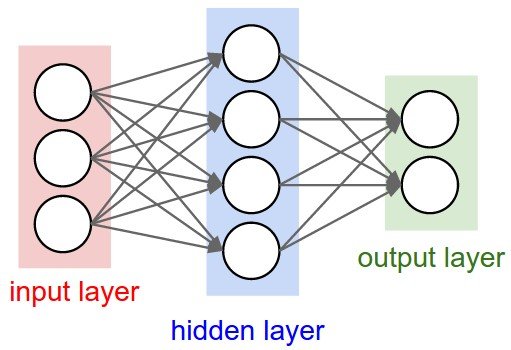
\includegraphics[width=0.4\textwidth]{neural_net.jpeg}
	\caption{Rappresentazione grafica di un Multilayer Perceptron}
\label{fig:MLP}
\end{figure}

Le connessioni fra due strati $x$ e $y$ di $n$ e $m$ neuroni rispettivamente, possono essere formalizzate come segue:

\begin{equation*}
	\left.\begin{aligned}[c]
		x &\in \mathbb{R}^{n \times 1} &\quad 
		y &\in \mathbb{R}^{m \times 1} \\
		W &\in \mathbb{R}^{m \times n} &\quad
		b &\in \mathbb{R}^{m \times 1} \\
	\end{aligned}\quad \right\}
	\;
	\begin{aligned}[c]
		y = \phi(Wx + b)
	\end{aligned}
\end{equation*}

Altra aggiunta che si può notare nella formalizzazione è la presenza di $\phi$ ovvero una funzione di attivazione che aggiunge non linearità al modello multistrato e permette alla rete di approssimare qualsiasi funzione, come dimostrato nel 1989 da Cybenko\cite{Cybenko1989}.
Le funzioni di attivazione, illustrate nella figura~\ref{fig:ACT}, possono essere di vario tipo, di seguito sono elencate le più importanti:

\begin{description}[leftmargin=!,labelwidth=\widthof{\bfseries Exponential Linear Unit (ELU)}]
\label{itm:relus}
	\item[Funzione Logistica] 
		${(1 + e^{-x})}^{-1}$
	\item[Tangente Iperbolica]
		$\tanh(x)$
	\item[Rectified Linear Unit (ReLU)]
		$\max(0,\, x)$
	\item[Leaky ReLU]
		$\max(0.01x,\, x)$
	\item[LReLU Parametrica]
		$\begin{cases}
			\alpha x &\text{se } x \geq 0 \\
			x &\text{se } x < 0 \\
		\end{cases}$
	\item[Exponential Linear Unit (ELU)]
		$\begin{cases}
			\alpha(e^x - 1) &\text{se } x \geq 0 \\
			x &\text{se } x < 0 \\
		\end{cases}$
\end{description}

\begin{figure}[H]
	\centering
	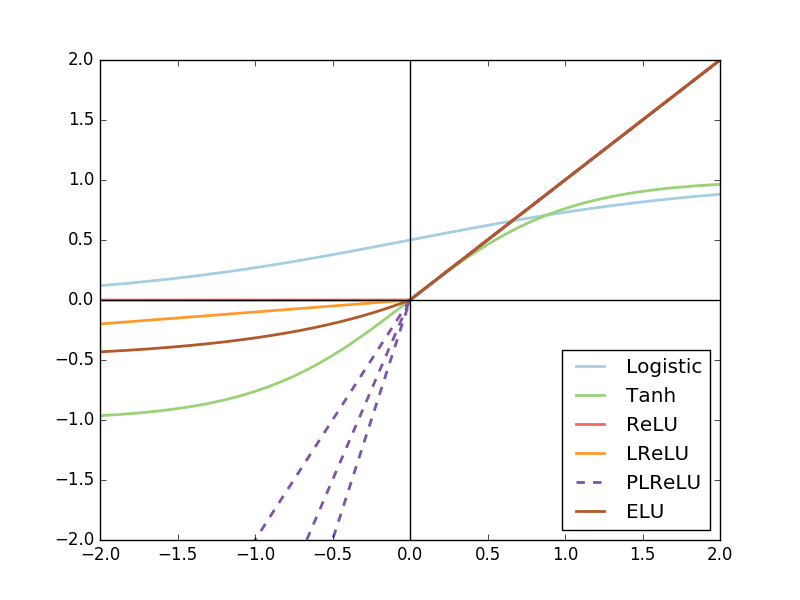
\includegraphics[width=0.6\textwidth]{activation_function.png}
	\caption{Comparazione fra le diverse funzioni di attivazione.}
\label{fig:ACT}
\end{figure}


Dato il modello appena descritto dunque non rimane che utilizzarlo come classificatore (con più di due classi e non-lineare a differenza del Perceptron di base) oppure per un task di regressione. Il prossimo passo è perciò quello di definire la funzione di costo (detta in gergo di \textit{Loss}) da utilizzare con l'algoritmo di backpropagation.


\subsection{Funzioni di Loss}

\subsubsection{Classificazione}
Assumiamo che ogni neurone $f_{j}$ del layer di output rappresenti uno score di appartenenza ad un certa classe e $y$ sia la classe a cui appartiene $x$:
\begin{description}
	\item[Hinge Loss]
		\quad\\$\Delta$ rappresenta la distanza minima richiesta di ogni score da quello della classe corretta.
		$$
		L = \sum_{j \neq{} y}{\max(0,\, {f_j} -{f_y} +\Delta)}
		$$
	\item[Softmax Cross-Entropy]
		\quad\\Con questo metodo lo score di ogni classe viene normalizzato. Il valore di loss finale è tanto minore quanto vicino a $1$ è la probabilità della classe corretta.
		$$
		L = -\log{\bigg(\frac{e^{f_y}}{\sum_j{e^{f_j}}}\bigg)}
		$$
\end{description}


\subsubsection{Regressione}
Assumiamo che ogni neurone $f_{i}$ del layer di output rappresenti una quantità da predire e $y$ sia un vettore dei valori attesi.

\begin{description}
	\item[L1 Loss]
		\quad\\Distanza di Manhattan.
		$$
		L = \Vert{f-y}\Vert_1 = \sum_{i}{\mid{f_i -y_i \mid}}
		$$
	\item[L2 Loss]
		\quad\\Distanza euclidea al quadrato per facilitare il calcolo della derivata durante la backpropagation.
		$$
		L = \Vert{f -y \Vert_2^2} = \sum_{i}{ (f_i -y_i)^2 }
		$$
\end{description}


\subsection{Apprendimento}

Ultimo passo per completare il meccanismo di apprendimento di una rete neurale è quello di definire come l'algoritmo di backpropagation dovrà aggiornare i valori dei vari neuroni.

Il metodo base della discesa stocastica del gradiente (SGD) opera come segue su un certo vettore $x$ di parametri al tempo $t+1$ utilizzando un \textit{learning rate} $\eta$ predefinito:
$$
x_{t+1} = x_t -\eta{} \cdot \frac{dL}{dx_t}
$$

In seguito verranno elencate diverse ottimizzazioni da poter usare insieme al metodo di base per accellerare il processo di apprendimento.\\
Ci riferiremo ai gradienti calcolati più semplicemente con:
$$dx_t = \frac{dL}{dx_t}$$

\subsubsection{Momentum Update}\cite{Momentum}
Viene aggiunto un ulteriore iperparametro $\alpha$ e una variabile $\Delta{x}$ in maniera da favorire la discesa in punti con alto gradiente.
\begin{align*}
	\Delta x_{t+1} &= \eta \cdot dx_t + \alpha \Delta x_t \\
	x_{t+1} &= x_t - \Delta x_{t+1}
\end{align*}

\subsubsection{Adagrad}\cite{Adagrad}
Learning rate adattivo per ogni singolo parametro grazie ad una variabile che tiene traccia del quadrato del gradiente.
\begin{align*}
	G_{x}^{(t+1)} &= G_x^{t} + dx_t^2 \\
	x_{t+1} &= x_t - \frac{\eta \cdot dx_t}{\sqrt{G_x^{(t+1)}} + \epsilon}
\end{align*}
\subsubsection{RMSProp}\cite{RMSProp}
Simile ad Adagrad con l'aggiunta di un iperparametro $\beta$ (decay rate) che previene la descrescenza monotonica del learning rate mantenendo una media mobile del quadrato del gradiente.
\begin{align*}
	G_x^{(t+1)} &= \beta \cdot G_x^t + (1 - \beta) \cdot dx_t^2 \\
	x_{t+1} &= x_t - \frac{\eta \cdot dx_t}{\sqrt{G_x^{(t+1)}} + \epsilon}
\end{align*}
\subsubsection{Adam}\cite{Adam}
Utilizza le medie mobili sia del gradiente che del suo quadrato introducendo dunque due iperparametri $\beta_1$ e $\beta_2$. Queste vengono in seguito corretti per evitare un annichilimento durante le prime iterazioni. 
\begin{align*}
	m_x^{(t+1)} &= \beta_1 \cdot m_t + (1-\beta_1) \cdot dx_t \quad&
	\hat{m}_x &= \frac{m_x^{(t+1)}}{1 - \beta_1^t} \\
	v_x^{(t+1)} &= \beta_2 \cdot v_t + (1-\beta_2) \cdot dx_t^2 \quad&
	\hat{v}_x &= \frac{m_x^{(t+1)}}{1 - \beta_2^t}
\end{align*}
$$
  x_{t+1} = x_t - \frac{\eta \cdot \hat{m}_x}{\sqrt{\hat{v}_x} + \epsilon}
$$

\subsection{Ottimizzazioni}

In questa sezione verranno discussi i principali metodi che consentono il miglioramento delle prestazioni di una qualsiasi rete neurale, sia dal punto di vista della velocità che della qualità dell'apprendimento.

\subsubsection{Data preprocessing}

Le principali operazioni sono quelle di sottrazione del \textit{valore medio} dall'intero campione di dati di training e la sua \textit{normalizzazione} attraverso la divisione per la deviazione standard. Queste operazioni permettono di avere dei dati geometricamente centrati all'origine e con valori compresi tra -1 e 1.


\subsubsection{Dropout}

Introdotto nel 2014\cite{dropout}, consiste nell'introdurre una probabilità $p$ che ogni neurone ha di rimanere attivo durante la fase di addestramento. L'obiettivo è quello di evitare l'overfitting dei dati attraverso epoche diverse.

\begin{figure}[H]
	\centering
	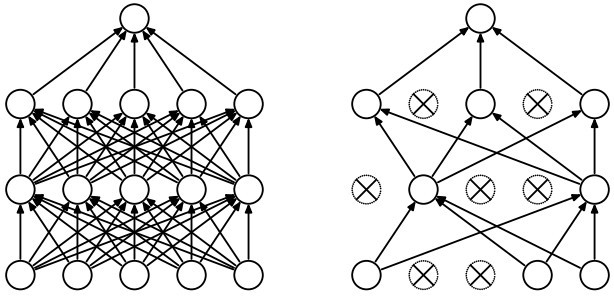
\includegraphics[width=0.6\textwidth]{dropout.jpeg}
	\caption{Rete neurale prima e dopo l'applicazione del dropout.}
\label{fig:dropout}
\end{figure}



\subsubsection{Inizializzazione dei pesi}

Dato che un'inizializzazione costante di tutti i pesi porterebbe a gradienti costanti, una soluzione consiste nell'utilizzare valori randomici prossimi a 0 distribuiti secondo una normale divisi per la radice quadrata del numero di input del layer. Ciò è dovuto dal fatto che un numero maggiore porterebbe ad una varianza sempre maggiore.
Dato però l'utilizzo di funzioni di attivazione, viene violata l'assunzione di una media nulla ed è dunque stata identificato il valore $\sqrt{2/n}$ come reale valore della varianza~\cite{he2015delving}.


\subsubsection{Batch Normalization}

Introdotta nel 2015\cite{batchnorm} con l'obiettivo di contrastare inizializzazioni sfavorevoli dei pesi nella rete, consiste nell'inserimento di un layer di normalizzazione tra ogni componente connessa e la relativa funzione di attivazione.


\section{Reti Neurali Convoluzionali}

Il modello di rete neurale visto fino ad ora rappresenta solamente le fondamenta degli strumenti odierni.
In seguito verranno dunque descritte le cosiddette \textit{CNN} in quanto modello principale che ha preso piede nel campo della Computer Vision.

\subsection{Struttura delle CNN}

Prima di illustrare le varie architetture che si son succedute negli anni è doveroso spiegare come si possa adattare un modello basato su \textit{fully-connected layers} (come per il Multilayer Perceptron visto nella sezione~\ref{subsec:mlp}) in modo da avere come input delle immagini (anche di dimensione diversa) evitando l'esplosione del numero di pesi da addestrare.

\subsubsection{Convolution Layer}
Ovvero il layer principale che dà il nome alle reti neurali convoluzionali.
L'idea principale è quella di avere $n$ filtri, solitamente di 3 o 5 pixel per lato, che vengono applicati all'input.
Gli iperparametri principali sono:
\begin{itemize}
	\item \textbf{Dimensione} del filtro.
	\item \textbf{Profondità}, il numero di filtri.
	\item \textbf{Stride}, di quanti pixel spostare il filtro.
	\item \textbf{Padding}, se aggiungere un bordo all'input per mantenere costante la dimensioni in output e nel caso quali valori usare.
\end{itemize}
\vspace{\fill}
\begin{figure}[H]
	\centering
	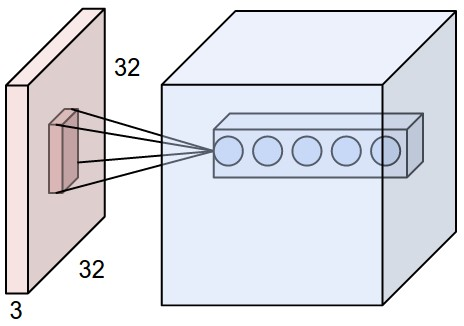
\includegraphics[width=0.4\textwidth]{convlayer.jpeg}
	\caption{Visualizzazione di un'operazione di convoluzione.}
\label{fig:convlayer}
\end{figure}

\subsubsection{ReLU Layer}
Applicazione delle funzioni di attivazione descritte nella sezione~\ref{itm:relus}.

\subsubsection{Pooling Layer}
Consente di ridurre la dimensione spaziale dell'input in base ad iperparametri $s$ stride e $n$ estensione del campo ricettivo.\\
I criteri di scelta del valore di output sono principalmente due: \textit{max pooling} (scelta del massimo) oppure \textit{average pooling} (scelta della media).\par

\subsubsection{Deconvolution Layer}
Non è altro che una convoluzione con stride frazionario che aumenta le dimensioni spaziali (de-pooling) dell'input ma che ne riduce la profondità invertendo dunque il \textit{forward pass} con il \textit{backward pass}.


\subsection{Breve storia}

\subsubsection{LeNet}

Nonostante già nel 1988~\cite{zhang1990parallel} vennero mossi i primi passi verso l'ideazione di un precursore delle reti convoluzionali, solo l'architettura ideata nel 1998 da LeCun et al.\cite{LeNet} viene oggi considerata come la prima vera \textit{CNN}.\par
Questo modello, introdotto con lo scopo di riconoscere caratteri scritti a mano, come mostrato in figura~\ref{fig:lenet5}, era composto da 4 sequenze di convoluzioni e ridimensionamenti, seguiti da 3 fully-connected layer ed una funzione a base radiale gaussiana finale per stimare gli errori per le singole classi.\par

\begin{figure}[H]
	\centering
	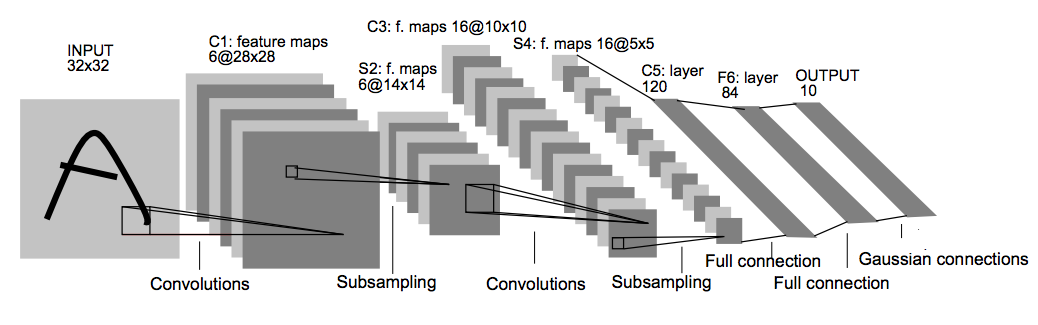
\includegraphics[width=0.9\textwidth]{lenet5.png}
	\caption{Schema di LeNet-5.}
\label{fig:lenet5}
\end{figure}

\subsubsection{GPGPU}
Questi sviluppi furono ancora osteggiati dall'elevata capacità computazionale richiesta per l'addestramento delle reti neurali. Nei primi anni del nuovo millennio infatti gli studi si concentrarono principalmente sullo studio di tecniche di addestramento attraverso l'utilizzo di \textit{Graphic Compute Units} in seguito alla pubblicazione di una ricerca nel 2005 che ne descriveva il loro valore nel campo del machine learning.\cite{gpuml}

\subsection{Casi di studio}
\label{subsec:case_studies}
Di seguito descriveremo velocemente diverse architetture sviluppatosi molto recentemente in seguito all'implementazione di LeNet su GPU nel 2011.\cite{gpu2011}

\subsubsection{AlexNet}
Questa rete neurale\cite{alexnet} è presentata in occasione della \textit{ImageNet ILSVRC Challenge}\cite{ILSVRC15} nel 2012, competizione annuale che prevedeva task di classificazione e localizzazione di ben 1000 classi differenti. Prendendo spunto direttamente da LeNet, questa architettura è riuscita a raggiungere risultati inimmaginabili sovraperformando il secondo classificato di ben 10 punti sulla percentuale d'errore.
\vfill
\begin{figure}[H]
	\centering
	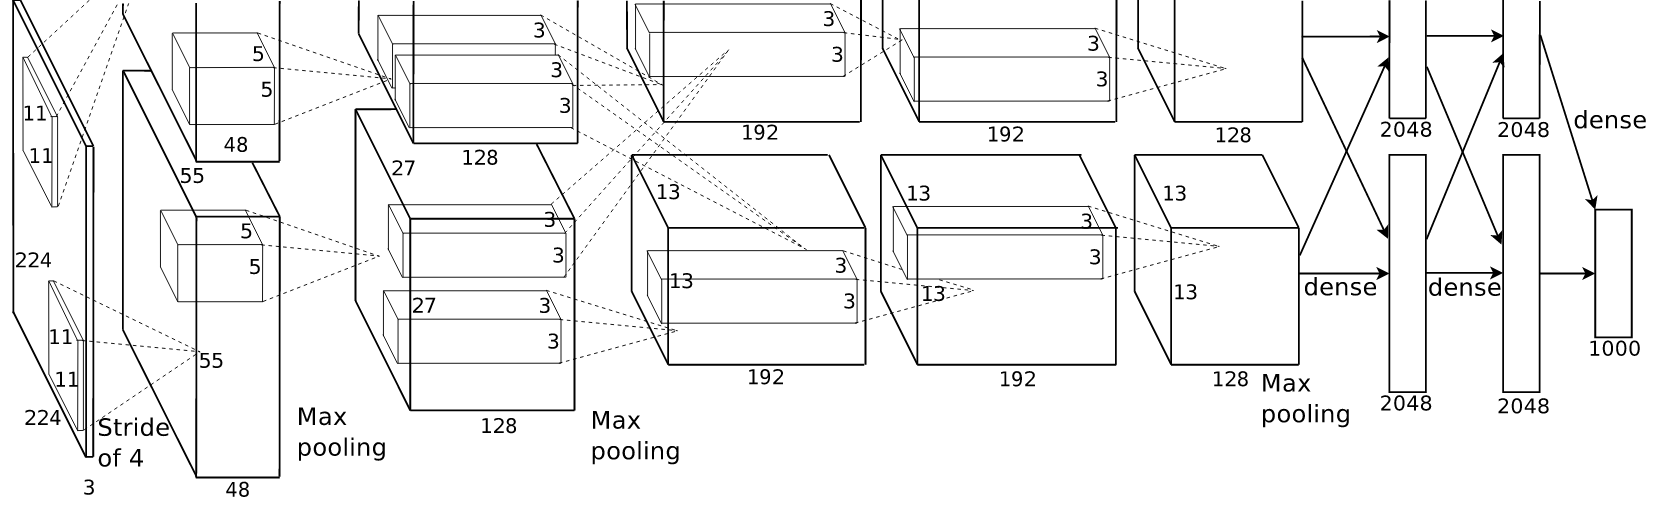
\includegraphics[width=\textwidth]{alexnet.png}
	\caption{Schema di AlexNet.}
\label{fig:alexnet}
\end{figure}
\vfill
\subsubsection{GoogLeNet}
Vincitrice dela \textit{ImageNet ILSVRC Challenge} nel 2014, ideata da Szegedy et al.\ da Google~\cite{googlenet}, ha introdotto il concetto di \textit{Inception Module}, illustrato in figura~\ref{fig:inception}, in maniera da ridurre drasticamente il numero di parametri (4 milioni rispetto ai 60 di AlexNet).

\begin{figure}[H]
	\centering
	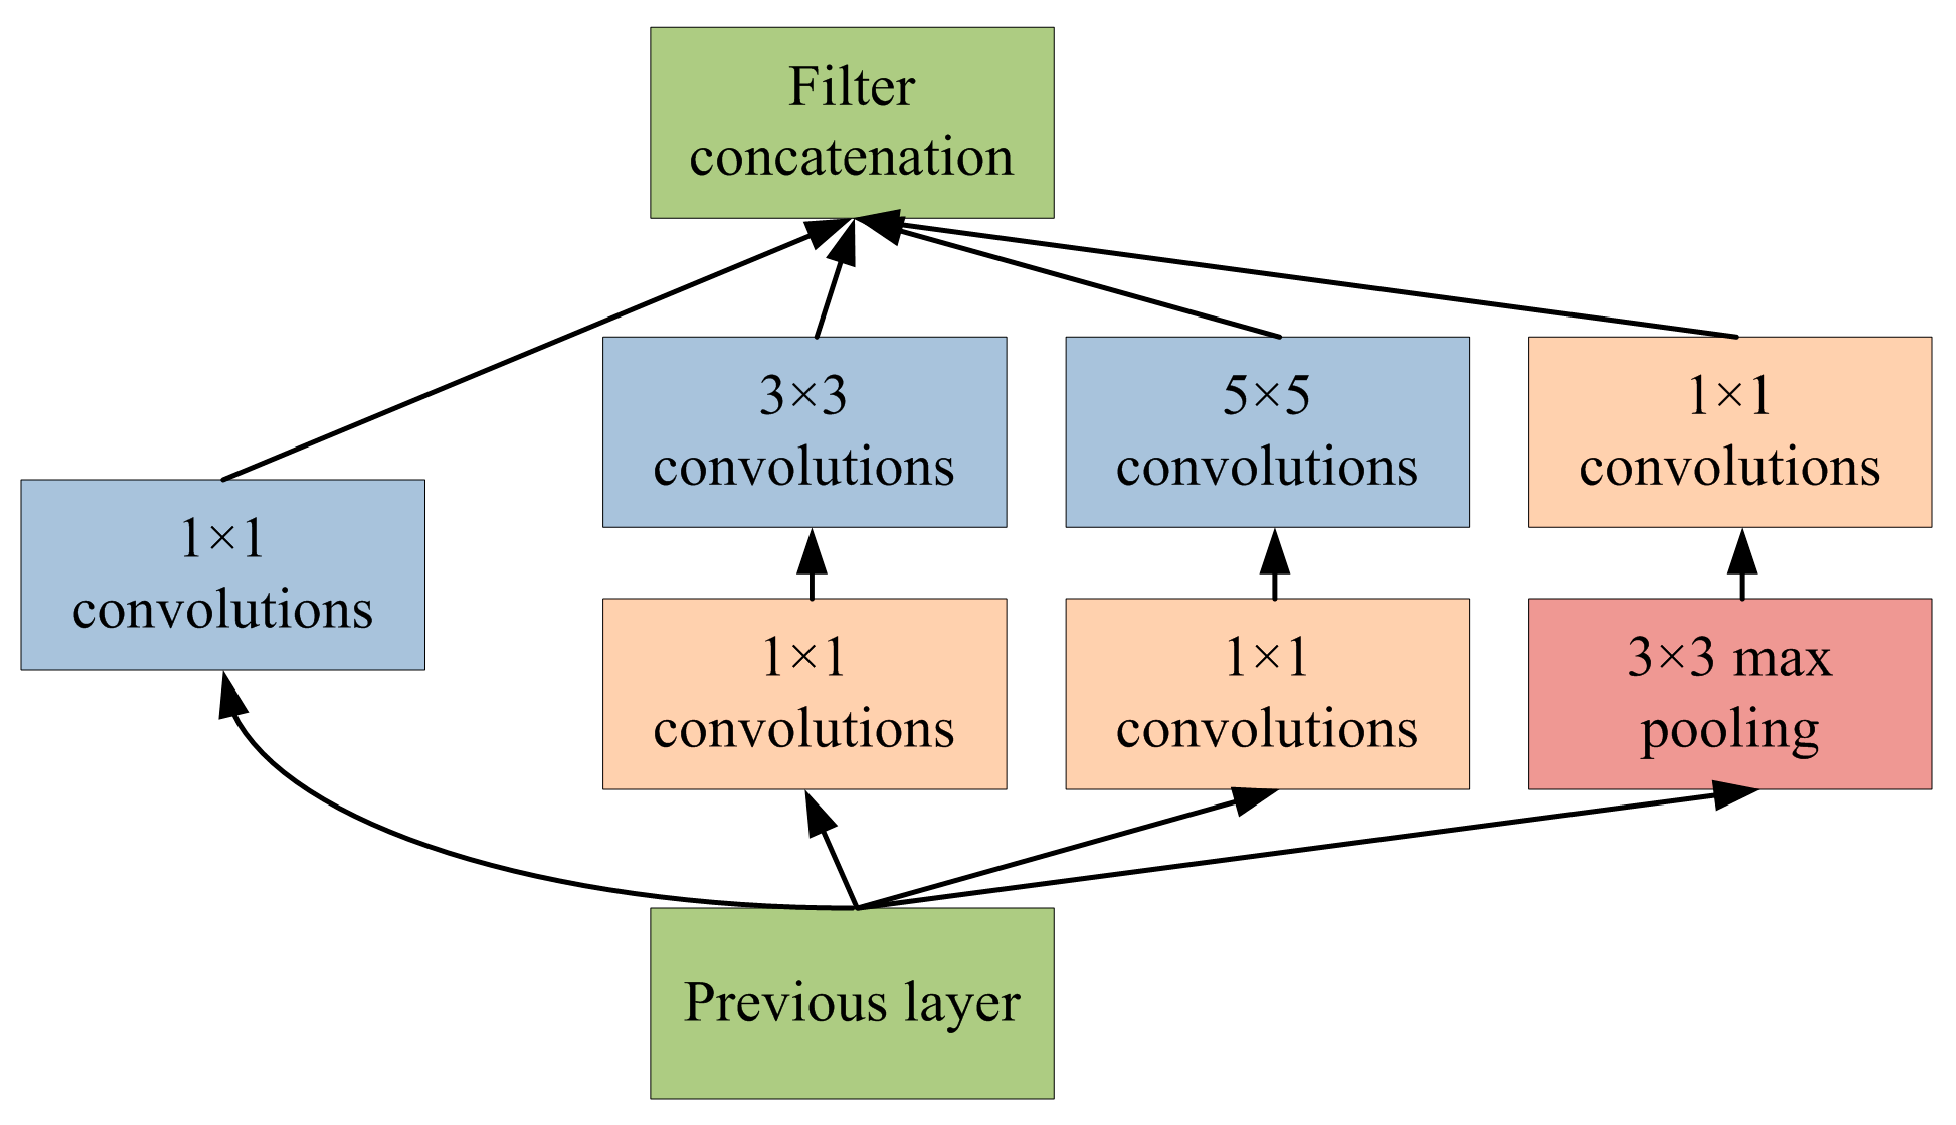
\includegraphics[width=0.6\textwidth]{inception_module.png}
	\caption{Inception Module di GoogLeNet.}
\label{fig:inception}
\end{figure}

\subsubsection{VGG}
Nonostante si è classificata solo in seconda posizione scontrandosi con GoogLeNet, questa architettura ideata da Karen Simonyan and Andrew Zisserman\cite{VGG} ha mostrato che la \textit{profondità} di una rete era una componenete principale per performance maggiori. Altro punto di forza è la sua semplicità strutturale nonostante il numero di parametri elevato, ben 140 milioni, dovuti agli ultimi fully-connected layer.
\begin{figure}[H]
	\centering
	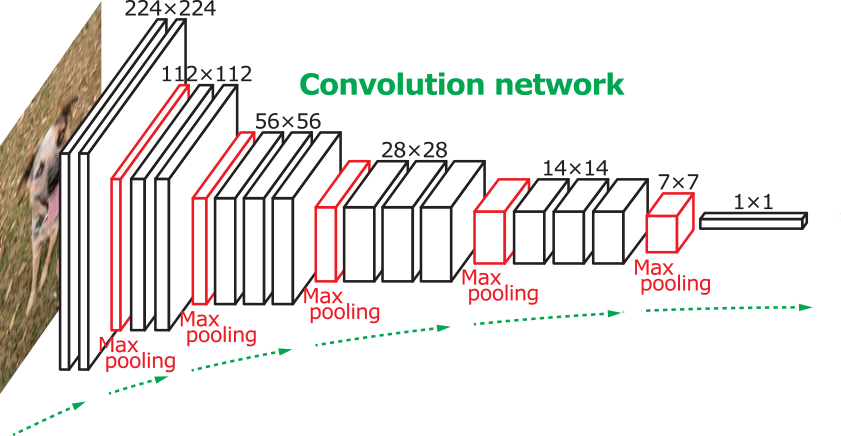
\includegraphics[width=0.75\textwidth]{vgg16.png}
	\caption{Schema di VGG16.}
\label{fig:vgg16}
\end{figure}

\subsubsection{ResNet}
\cite{resnet}Vincitrice di \textit{ILSVRC Challenge 2015}, introduce le cosiddette \textit{Shortcut Connections}, illustrate in figura~\ref{fig:residual}, in modo da risolvere il problema della degradazione del segnale di errore in reti molto profonde.

\begin{figure}[H]
	\centering
	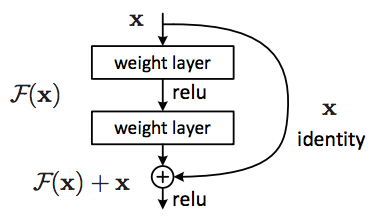
\includegraphics[width=0.5\textwidth]{residual_block.png}
	\caption{Shortcut Connection.}
\label{fig:residual}
\end{figure}


\section{Fully Convolutional Network}
\label{sec:FCN}
Tutte le architetture citate in precedenza per quanto potenti ed innovative, nella loro configurazione di base sono solo atte a classificare un'immagine, ovvero a fornire le probabilità di appartenenza a ciascuna classe su cui sono state addestrate.\par
Questa limitazione perciò non ci permette di eseguire classificazioni multiple o localizzazioni, per esempio separare due oggetti appartenenti alla stessa classe oppure rilevare due oggetti di due classi differenti all'interno di una stessa immagine.\par
Per la localizzazione singola di una classe una soluzione banale è quella di passare da un task di classificazione ad uno di regressione delle coordinate della bounding box cambiando dunque la funzione di loss finale.\par
Negli anni si sono avuti ulteriori raffinamenti atti a compensare queste lacune, dapprima con FastRCNN\cite{fastrcnn} ed il successivo FasterRCNN\cite{fasterrcnn} e più recentemente con YOLO\cite{yolo}, tutti nati con lo scopo di predire bounding box multiple con rispettive classi di appartenenza. Quello però di cui tratteremo in questa sezione è un approccio completamente differente.\par
Ideata nel 2014~\cite{fcn}, una \textit{Fully Convolutional Network} si pone l'obiettivo di generare un output della stessa dimensione dell'immagine di input in cui ogni pixel rappresenta la propria classe di appartenenza, praticamente semgentando l'immagine originale.\par
Grande pregio di questa architettura è la propria semplicità strutturale, infatti, come mostrato in figura~\ref{fig:fcn}, non fa altro che riprendere la \textit{VGG16} ed ampliarla aggiungendo uno o più layer di deconvoluzione addizionati ai precedenti output dei layer di pooling per generare l'immagine finale.

\begin{figure}[H]
	\centering
	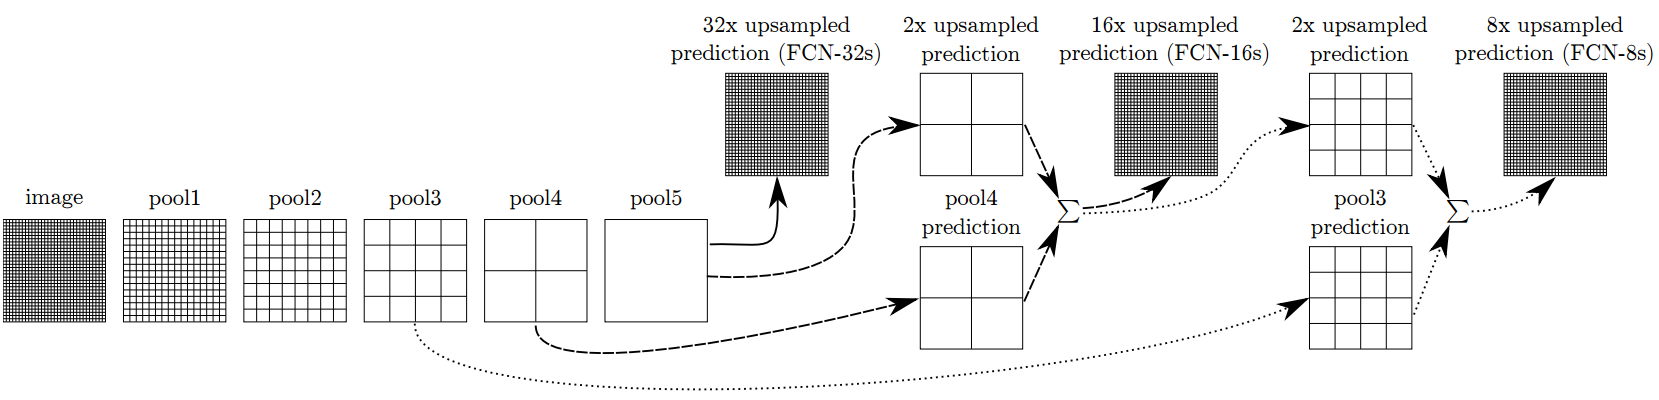
\includegraphics[width=\textwidth]{fcn.png}
	\caption{Schema delle Fully Convolutional Network.}
\label{fig:fcn}
\end{figure}

